\section{逼近误差}
\label{sec:fapprox-error}

上一节说“存在误差小于$\varepsilon$的近似”，却允许近似的复杂程度随$\varepsilon$任意增长。回到章首的投影图景：要谈“替身离目标多远”，先要定下目标、尺子和允许的候选集合。本节先用候选集合定义最佳可能误差，把它同具体构造得到的误差分开；再比较候选集合是否为线性子空间、尺子是否由内积给出；最后用Fourier截断，把“丢掉坐标”的代价逐项算出来。

\subsection{目标、误差与表示预算}
\label{sec:fapprox-budget}

设$X$是赋范函数空间，$f\in X$是目标。对每个预算$N$，规定一个候选集合$\mathcal A_N\subseteq X$，它包含所有“用预算$N$能写出的函数”。预算可以是线性子空间的维数，可以是展开中允许保留的项数，也可以是分段函数的段数。

要比较候选集合的好坏，最公平的度量是其中最好的那个候选能做到多好。下面的定义就是把点到集合的距离搬到函数上。

\begin{definition}[最佳逼近误差]
\label{def:fapprox-best-error}
对$f\in X$与候选集合$\mathcal A_N\subseteq X$，称
\begin{equation}
 E(f,\mathcal A_N)_X=\inf_{g\in\mathcal A_N}\lVert f-g\rVert_X
 \label{eq:fapprox-best-error}
\end{equation}
为$f$在$\mathcal A_N$中的\term{最佳逼近误差}（error of best approximation）。
\end{definition}

这就是第~\ref{chap:metric-spaces}章的点到集合的距离。由那里的序列判据，$E(f,\mathcal A_N)_X=0$当且仅当$f$属于$\mathcal A_N$的闭包。若$\mathcal A_N$随$N$递增且并集稠密，上一节的结论就可以重述为$E(f,\mathcal A_N)_X\to0$。

最佳误差是在所有候选中取下确界，不依赖任何具体的选法。某个具体构造（例如在结点处插值）得到的误差只是它的一个上界。后面要反复区分这两者。

\paragraph{三种预算}
三种常见预算给出性质不同的候选集合。次数小于$N$的多项式组成$N$维线性空间，好比$\mathbb R^n$中一张固定的$N$维平面。

给定一组标准正交基后，至多用其中$N$个基向量的线性组合组成的集合就不同了。$\mathbb R^2$中$N=1$时，它是两条坐标轴的并，不是平面也不是直线；$e_1$与$e_2$都只用一项，和$e_1+e_2$却要两项。区间上至多$N$段的分段常数函数，若分点可以任意移动，同样不对加法封闭。

后两种集合对数乘封闭，但对加法不封闭，相应的逼近称为\term{非线性逼近}（nonlinear approximation），以区别于在固定线性空间中进行的线性逼近。

\paragraph{单个函数与函数类}
有时我们要的不是某一个函数的误差，而是对一整类函数$\mathcal F$同时有效的保证。此时考虑最坏情形
\begin{equation}
 E(\mathcal F,\mathcal A_N)_X=\sup_{f\in\mathcal F}E(f,\mathcal A_N)_X .
 \label{eq:fapprox-worst-case}
\end{equation}

两者可以相差很多，这也是无限维与有限维差别最明显的地方。设$H$是可分无限维Hilbert空间，$(e_n)$为标准正交基，$V_N=\operatorname{span}\{e_1,\ldots,e_N\}$。对每个$f$，有
\[
 E(f,V_N)^2=\sum_{n>N}\lvert\langle e_n,f\rangle\rvert^2\to0 .
\]
可是对闭单位球$\mathcal F$，取$f=e_{N+1}$，它与$V_N$垂直，距离为$1$，所以
\[
 E(\mathcal F,V_N)=1\qquad\text{对每个}\ N.
\]
单个函数的误差都趋于零，整个单位球却没有共同的速率。在$\mathbb R^n$中，取$V_n$就把全空间装下了，这种现象不会发生。

要得到统一速率，函数类本身必须足够“小”。这与第~\ref{chap:function-class-covers}章的有限覆盖直接相关：若候选集合$\mathcal A$是至多$N$个函数组成的有限集，最坏误差不超过$\varepsilon$恰好说明以$\mathcal A$中各点为中心、半径为$\varepsilon$的闭球覆盖$\mathcal F$。

反过来，若$\mathcal F$能被$N$个半径为$\varepsilon$的闭球覆盖，以这些球心为$\mathcal A$，最坏误差就不超过$\varepsilon$。覆盖数因此恰好描述了用$N$个固定函数逼近整个函数类所能达到的最坏误差。

\subsection{固定空间中的最佳逼近}
\label{sec:fapprox-fixed-space}

最常见的预算是维数。取一列嵌套的有限维子空间$V_1\subseteq V_2\subseteq\cdots\subseteq X$，$\dim V_N\leq N$，研究$E(f,V_N)_X$。一个基本的问题是：下确界能否取到，也就是最近点是否存在。

\begin{theorem}[有限维子空间中最佳逼近的存在]
\label{thm:fapprox-existence}
设$X$为赋范空间，$V\subseteq X$为有限维子空间，$f\in X$。则存在$g^*\in V$使$\lVert f-g^*\rVert=E(f,V)_X$。
\end{theorem}

\begin{proof}
记$d=E(f,V)_X$，取$g_n\in V$使$\lVert f-g_n\rVert\to d$。$n$充分大时，$\lVert f-g_n\rVert\leq d+1$，于是
\[
 \lVert g_n\rVert\leq\lVert f\rVert+\lVert f-g_n\rVert\leq\lVert f\rVert+d+1 .
\]
$(g_n)$是有限维空间中的有界序列。有限维赋范空间中有界闭集是紧集，所以有子列收敛到某个$g^*\in V$。范数连续，取极限得
\[
 \lVert f-g^*\rVert=\lim_k\lVert f-g_{n_k}\rVert=d .
\]
\end{proof}

证明的关键是有限维的闭球紧。这个定理对$V$的维数有实质要求：无限维子空间中最近点可能不存在，第~\ref{chap:function-inner-product-spaces}章用完备性和平行四边形恒等式才在Hilbert空间中重新得到它。

存在不等于唯一，尺子的形状决定了最近点的个数。在$\mathbb R^2$上取最大值范数（两个分量绝对值的较大者），$V=\operatorname{span}\{(0,1)\}$，$f=(1,0)$。对候选$(0,t)$，
\[
 \lVert f-(0,t)\rVert_\infty=\max\{1,\lvert t\rvert\},
\]
对所有$\lvert t\rvert\leq1$都取到最小值$1$，最佳逼近有无穷多个。

图~\ref{fig:fapprox-nearest-point}说明了原因。以$f$为中心把球吹大，第一次碰到$V$的地方就是最近点。欧氏球是圆，碰到直线只有一点；最大值范数的球是正方形，它的一条边整个贴上了直线。

\begin{BookInlineFigure}
  \centering
  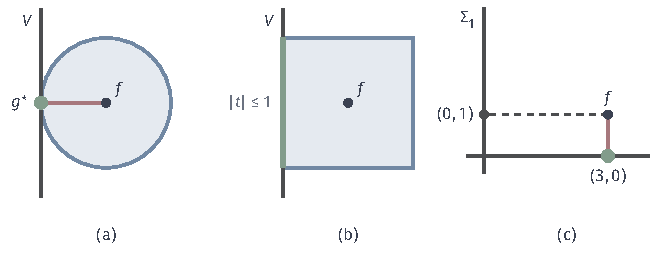
\includegraphics[width=110.882mm]{figures/04-spaces-measures-and-geometry/03-function-spaces/tikz/fapprox-nearest-point/figure.pdf}
  \caption{候选集合与尺子决定最近点。(a)$\mathbb R^2$中欧氏范数：以$f=(1,0)$为中心的圆第一次碰到直线$V$时只有一个切点$g^*$（绿）。(b)最大值范数：同样的半径下，球是正方形，整条边$\{(0,t):\lvert t\rvert\leq1\}$（绿）都是最近点。(c)候选集合$\Sigma_1$是两条坐标轴的并，并非子空间；对$f=(3,1)$，到横轴的距离$1$（红）小于到纵轴的距离$3$（虚线），最近点是$(3,0)$。}
  \label{fig:fapprox-nearest-point}
\end{BookInlineFigure}

\paragraph{Hilbert空间中的正交投影}
内积给出的尺子最好用。由第~\ref{chap:function-inner-product-spaces}章，对闭子空间$V$，正交投影$P_V$给出唯一的最佳逼近，误差满足勾股关系
\begin{equation}
 E(f,V)^2=\lVert f-P_Vf\rVert^2=\lVert f\rVert^2-\lVert P_Vf\rVert^2 .
 \label{eq:fapprox-pythagoras}
\end{equation}
若$V$有标准正交基$e_1,\ldots,e_N$，则投影公式就是把分量读出来：
\[
 P_Vf=\sum_{n\leq N}\langle e_n,f\rangle e_n .
\]
映射$f\mapsto P_Vf$是线性的，这正是后面截断误差可以逐项计算的原因。

\begin{example}[把$x^2$投影到一次函数]
在$L^2[0,1]$中，用次数不超过$1$的多项式逼近$f(x)=x^2$。这个二维子空间有标准正交基
\[
 e_1(x)=1,\qquad e_2(x)=\sqrt{12}\Bigl(x-\frac12\Bigr).
\]

读出$f$在两个方向上的分量：
\[
 \langle e_1,f\rangle=\frac13,\qquad
 \langle e_2,f\rangle=\sqrt{12}\Bigl(\frac14-\frac16\Bigr)=\frac1{\sqrt{12}}.
\]
代入投影公式，$\sqrt{12}$约去，
\[
 P_Vf(x)=\frac13+x-\frac12=x-\frac16 .
\]

误差由式~\eqref{eq:fapprox-pythagoras}得到，只需做减法，这和$\mathbb R^3$中用勾股定理求点到平面的距离一样：
\[
 E(f,V)^2=\frac15-\frac19-\frac1{12}=\frac1{180}.
\]
\end{example}

\paragraph{不同的尺子，不同的最佳近似}
在其他范数下，最佳逼近的结果和性质都会变。在$C[0,1]$中用常数作一致逼近：若$f$的最大值、最小值分别是$M,m$，则
\[
 \max_x\lvert f(x)-c\rvert=\max\{M-c,\ c-m\}.
\]
两项一增一减，取$c=(M+m)/2$时相等，最小。所以唯一的最佳常数和最佳误差是
\begin{equation}
 c^*=\frac{M+m}2,\qquad E=\frac{M-m}2 .
 \label{eq:fapprox-best-constant}
\end{equation}

对比$L^2[0,1]$中的最佳常数，它是在一维子空间$\operatorname{span}\{1\}$上的投影，等于平均值。取$f(x)=x^2$，两种尺子给出不同的答案：
\[
 c_{L^2}=\int_0^1x^2\,\mathrm dx=\frac13,\qquad c_\infty=\frac{1+0}2=\frac12 .
\]

一致逼近的最佳选择甚至不是线性的。取$f_1(x)=x$，最佳常数为$1/2$；取$f_2(x)=-x^2$，最佳常数为$-1/2$；而$f_1+f_2=x-x^2$的最大值$1/4$、最小值$0$，最佳常数为$1/8$，不等于$\frac12+(-\frac12)=0$。所以在线性空间中选近似，并不意味着“选出最佳近似”这个操作本身是线性的。第~\ref{sec:fapprox-adaptive}节的分段常数逼近要用到式~\eqref{eq:fapprox-best-constant}。

\subsection{正交展开的截断误差}
\label{sec:fapprox-fourier-truncation}

Hilbert空间中，若嵌套空间由一组标准正交基的前若干项张成，最佳误差就是被舍弃分量的平方和，和$\mathbb R^3$中丢掉第三个分量完全一样。Fourier级数是最重要的例子。本小节在$L^2(0,1)$上采用周期为$1$的基：
\[
 e_k(x)=\mathrm e^{2\pi\mathrm ikx},\qquad k\in\mathbb Z ,
\]
函数$f$在第$k$个方向上的分量是
\[
 \hat f(k)=\langle e_k,f\rangle=\int_0^1f(x)\mathrm e^{-2\pi\mathrm ikx}\,\mathrm dx .
\]
第~\ref{chap:fourier-transform}章对周期$2\pi$的基建立了完备性，作线性变量代换后，$(e_k)_{k\in\mathbb Z}$是$L^2(0,1)$的标准正交基，Parseval等式$\lVert f\rVert_2^2=\sum_k\lvert\hat f(k)\rvert^2$成立。

\paragraph{平方误差与保留维数}
保留$\lvert k\rvert\leq K$的项，令$P_Kf=\sum_{\lvert k\rvert\leq K}\hat f(k)e_k$。它是到$2K+1$维空间$\operatorname{span}\{e_k:\lvert k\rvert\leq K\}$的正交投影。由Parseval等式，
\begin{equation}
 \lVert f-P_Kf\rVert_2^2=\sum_{\lvert k\rvert>K}\lvert\hat f(k)\rvert^2 .
 \label{eq:fapprox-fourier-tail}
\end{equation}
截断误差完全由分量的衰减决定，而衰减速度反映目标的正则性。下面用一个跳跃的函数和一个连续但有折点的函数比较。

第一个是锯齿函数$f(x)=x$，周期延拓后在整数点跳跃。$k=0$时积分是$1/2$。$k\neq0$时分部积分，
\[
 \hat f(k)=\Bigl[\frac{x\,\mathrm e^{-2\pi\mathrm ikx}}{-2\pi\mathrm ik}\Bigr]_0^1+\frac1{2\pi\mathrm ik}\int_0^1\mathrm e^{-2\pi\mathrm ikx}\,\mathrm dx .
\]
第二项的积分是零，第一项的上限给出
\[
 \hat f(k)=\frac1{-2\pi\mathrm ik}=\frac{\mathrm i}{2\pi k}.
\]
代入式~\eqref{eq:fapprox-fourier-tail}，并把$\pm k$的两项合并，
\[
 \lVert f-P_Kf\rVert_2^2=\frac1{2\pi^2}\sum_{k>K}\frac1{k^2}.
\]
这个尾和约为$1/K$，误差约为$(2\pi^2K)^{-1/2}$。实际计算得$K=10$时$\lVert f-P_Kf\rVert_2=0.0694$，$K=40$时为$0.0354$。项数增至四倍，误差只减半。

第二个是三角波$f_*(x)=\lvert x-\frac12\rvert$，周期延拓后连续，只有折点。$k=0$时积分是$1/4$。$k\neq0$时作代换$x=\frac12+t$，因子$\mathrm e^{-\pi\mathrm ik}=(-1)^k$提到积分外，$\lvert t\rvert$是偶函数，只留下余弦部分：
\[
 \hat f_*(k)=2(-1)^k\int_0^{1/2}t\cos(2\pi kt)\,\mathrm dt .
\]
再分部积分一次，
\[
 \int_0^{1/2}t\cos(2\pi kt)\,\mathrm dt=\frac{(-1)^k-1}{4\pi^2k^2}.
\]
合起来，并用$(-1)^{2k}=1$，
\[
 \hat f_*(k)=\frac{1-(-1)^k}{2\pi^2k^2}\qquad(k\neq0).
\]
奇数$k$时系数为$1/(\pi^2k^2)$，偶数$k$时为零。由式~\eqref{eq:fapprox-fourier-tail}，平方误差是
\[
 \lVert f_*-P_Kf_*\rVert_2^2=\frac2{\pi^4}\sum_{\substack{k>K\\k\ \text{奇}}}\frac1{k^4}\leq\frac2{3\pi^4K^3},
\]
不等号把尾和换成积分$\int_K^\infty t^{-4}\,\mathrm dt$来控制。$K=10$时实际误差为$0.00183$。系数从$k^{-1}$变成$k^{-2}$，误差的速率就从$K^{-1/2}$提高到$K^{-3/2}$。

多变量时，同样的截断在$[0,1)^d$上使用基
\[
 e_{\bm k}(\bm x)=\mathrm e^{2\pi\mathrm i\bm k\cdot\bm x},\qquad \bm k\in\mathbb Z^d .
\]
保留$\max_i\lvert k_i\rvert\leq K$的项需要$(2K+1)^d$个系数，保留$\lvert\bm k\rvert_2\leq K$的项大约需要半径为$K$的$d$维球体积那么多个系数。例如$d=2$、$K=10$时，前者是$441$个，后者是$317$个。比较误差时必须写明预算计的是哪一种。

\paragraph{一致误差}
平方误差小不等于每一点误差都小。设系数绝对可和，即
\[
 \sum_k\lvert\hat f(k)\rvert<\infty ,
\]
则级数$\sum_k\hat f(k)e_k$一致收敛到一个连续函数$\tilde f$。$\tilde f$与$f$有相同的Fourier系数，由Parseval等式，两者几乎处处相等。这个连续代表满足
\begin{equation}
 \sup_x\bigl\lvert\tilde f(x)-P_Kf(x)\bigr\rvert\leq\sum_{\lvert k\rvert>K}\lvert\hat f(k)\rvert .
 \label{eq:fapprox-uniform-tail}
\end{equation}

三角波的系数绝对可和，右端为
\[
 \frac2{\pi^2}\sum_{\substack{k>K\\k\ \text{奇}}}\frac1{k^2}\leq\frac2{\pi^2K}.
\]
在$x=1/2$处$e_k(1/2)=(-1)^k$，所有被舍弃的项同号，所以式~\eqref{eq:fapprox-uniform-tail}在这一点取等号，一致误差恰好等于这个尾和。$K=10$时它是$0.0101$。

锯齿函数的系数不绝对可和。$f$在整数点跳跃，而$P_Kf$连续，在跳跃点两侧的误差不可能都小于跳跃幅度的一半，所以一致误差不趋于零。图~\ref{fig:fapprox-fourier-truncation}(a)中，$P_{10}f$在跳跃附近摆动，其余地方已经贴近$f$。

两种误差的控制方式不同：平方误差用平方尾和，一致误差用绝对尾和，后者要求系数衰减得更快。图~\ref{fig:fapprox-fourier-truncation}(b)显示，三角波的平方误差按$K^{-3/2}$下降，一致误差只按$K^{-1}$下降。同一个截断，换一把尺子，所需的正则性和得到的速率都不同。

\begin{BookInlineFigure}
  \centering
  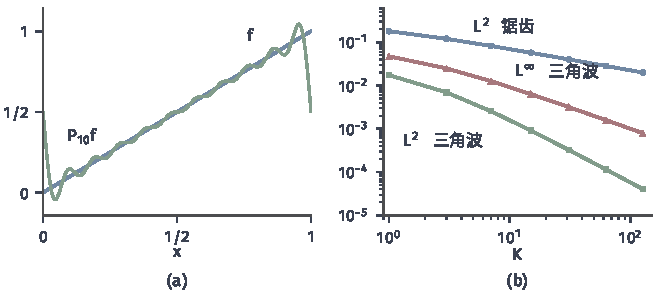
\includegraphics[width=112mm]{figures/04-spaces-measures-and-geometry/03-function-spaces/matplotlib/fapprox-fourier-truncation/figure.pdf}
  \caption{Fourier截断的误差。(a)锯齿函数$f(x)=x$（蓝）与截断$P_{10}f$（绿）。(b)误差随截断半径$K$的变化，双对数坐标，$K=1,3,7,\ldots,127$：锯齿函数的$L^2$误差按$K^{-1/2}$下降，三角波$\lvert x-\frac12\rvert$的$L^2$误差按$K^{-3/2}$下降，三角波的$L^\infty$误差按$K^{-1}$下降。}
  \label{fig:fapprox-fourier-truncation}
\end{BookInlineFigure}

\paragraph{理论截断与离散计算}
$P_Kf$中的系数是积分，实际计算时常用$M$个等距采样点上的求和代替：
\[
 \hat f_M(k)=\frac1M\sum_{j=0}^{M-1}f\Bigl(\frac jM\Bigr)\mathrm e^{-2\pi\mathrm ikj/M}.
\]
这相当于只读长向量上$M$个位置的分量，再用这$M$个数去估计频率坐标。$M$个数放不下无限多个频率坐标，必有信息被折叠到一起。

设系数绝对可和，在采样点使用连续代表$\tilde f=\sum_l\hat f(l)e_l$。把它代入上式，交换有限和与绝对收敛级数，内层出现的是几何和
\[
 \frac1M\sum_{j=0}^{M-1}\mathrm e^{2\pi\mathrm i(l-k)j/M}=
 \begin{cases}
  1,&l\equiv k\pmod M,\\
  0,&\text{其他情形}.
 \end{cases}
\]
于是
\begin{equation}
 \hat f_M(k)=\sum_{m\in\mathbb Z}\hat f(k+mM) .
 \label{eq:fapprox-aliasing}
\end{equation}
离散系数把所有与$k$模$M$同余的频率叠加在一起，这一现象称为\term{混叠}（aliasing）。

用三角波验证一下。取$M=4$，$k=1$，采样值依次是
\[
 f_*(0)=\frac12,\quad f_*\Bigl(\frac14\Bigr)=\frac14,\quad f_*\Bigl(\frac12\Bigr)=0,\quad f_*\Bigl(\frac34\Bigr)=\frac14 .
\]
指数因子依次是$1,-\mathrm i,-1,\mathrm i$，$j=1,3$两项相消，得到
\[
 \hat f_4(1)=\frac14\cdot\frac12=\frac18 .
\]

另一方面，$k+4m$取遍$\ldots,-7,-3,1,5,9,\ldots$，它们的绝对值恰好取遍所有正奇数各一次。由式~\eqref{eq:fapprox-aliasing}和$\sum_{n\ \text{奇},\,n>0}n^{-2}=\pi^2/8$，
\[
 \sum_{m\in\mathbb Z}\hat f_*(1+4m)=\frac1{\pi^2}\sum_{\substack{n>0\\n\ \text{奇}}}\frac1{n^2}=\frac18 ,
\]
两边相同。真实系数$\hat f_*(1)=1/\pi^2\approx0.1013$，被混入的高频抬高到了$0.125$。图~\ref{fig:fapprox-aliasing}(a)展示了混叠的机制，(b)展示了哪些频率被叠到一起。

\begin{BookInlineFigure}
  \centering
  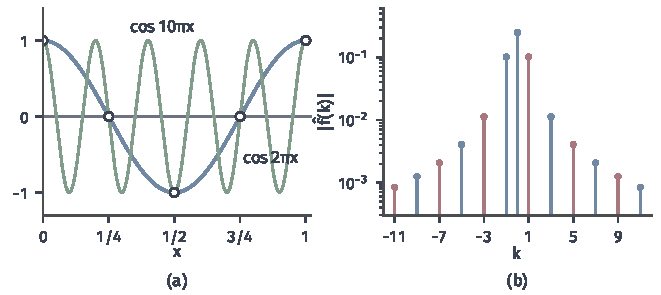
\includegraphics[width=112mm]{figures/04-spaces-measures-and-geometry/03-function-spaces/matplotlib/fapprox-aliasing/figure.pdf}
  \caption{$M=4$时的混叠。(a)$\cos2\pi x$（蓝）与$\cos10\pi x$（绿）在四个采样点$j/4$（空心圆）上取值相同，只看采样值无法区分频率$1$与$5$。(b)三角波系数的绝对值（对数纵轴）。红色频率$k\equiv1\pmod4$的系数相加，得到离散系数$\hat f_4(1)=1/8$；蓝色为其余频率。}
  \label{fig:fapprox-aliasing}
\end{BookInlineFigure}

用离散系数作截断时，误差有两个来源。设$g=\sum_{\lvert k\rvert\leq K}\hat f_M(k)e_k$，$f-g$分成互相正交的两部分：一部分在被舍弃的频率上，一部分在保留的频率上。勾股定理给出
\begin{equation}
 \lVert f-g\rVert_2^2=\sum_{\lvert k\rvert>K}\lvert\hat f(k)\rvert^2+\sum_{\lvert k\rvert\leq K}\lvert\hat f_M(k)-\hat f(k)\rvert^2 .
 \label{eq:fapprox-discrete-error}
\end{equation}

第一项是理论截断误差，只由$K$决定。第二项是离散误差，由式~\eqref{eq:fapprox-aliasing}知$\hat f_M(k)-\hat f(k)=\sum_{m\neq0}\hat f(k+mM)$，依赖采样数$M$与高频系数。两者应分别预算：增大$K$而不增大$M$，第二项不会减小；$2K+1>M$时，$M$个数据被重复计入不同的频率，增加保留项还会使离散误差变大。

\subsection{连续频带截断}
\label{sec:fapprox-band-truncation}

非周期函数没有离散频率，向量的“分量”换成了连续下标$\xi$上的$\hat f(\xi)$。相应的预算改为一段连续频带。在$L^2(\mathbb R)$上沿用第~\ref{chap:fourier-transform}章的归一化
\[
 \hat f(\xi)=\int_{\mathbb R}f(x)\mathrm e^{-2\pi\mathrm ix\xi}\,\mathrm dx ,
\]
先对$L^1\cap L^2$定义，再延拓到$L^2$。Plancherel等式是$\lVert\hat f\rVert_2=\lVert f\rVert_2$。

给定频带半宽$W>0$，令$Q_Wf$为$\hat f\mathbf 1_{[-W,W]}$的逆变换。乘以示性函数是$L^2$上的正交投影，Fourier变换是保持内积的双射，所以$Q_W$是到闭子空间
\[
 \mathcal B_W=\bigl\{g\in L^2(\mathbb R):\ \hat g=0\ \text{在}\ [-W,W]\ \text{外几乎处处成立}\bigr\}
\]
的正交投影。$\mathcal B_W$中的函数称为\term{带限函数}（band-limited function）。$Q_Wf$是$f$在$\mathcal B_W$中的最佳$L^2$逼近，由Plancherel等式，
\begin{equation}
 \lVert f-Q_Wf\rVert_2^2=\int_{\lvert\xi\rvert>W}\lvert\hat f(\xi)\rvert^2\,\mathrm d\xi .
 \label{eq:fapprox-band-tail}
\end{equation}

以Gauss函数$f(x)=\mathrm e^{-\pi x^2}$为例，$\hat f(\xi)=\mathrm e^{-\pi\xi^2}$。在积分区域上$\lvert\xi\rvert/W\geq1$，乘上这个因子可以把尾积分算出来：
\[
 \int_{\lvert\xi\rvert>W}\mathrm e^{-2\pi\xi^2}\,\mathrm d\xi\leq\frac2W\int_W^\infty\xi\,\mathrm e^{-2\pi\xi^2}\,\mathrm d\xi=\frac{\mathrm e^{-2\pi W^2}}{2\pi W}.
\]
$W=1$时误差$\lVert f-Q_Wf\rVert_2$约为$0.0167$，$W=1.5$时约为$2.7\times10^{-4}$。把右端的界开平方，分别得到$0.0172$与$2.8\times10^{-4}$，几乎与实际值一致。光滑而快速衰减的函数，频域尾部下降极快。

与上一小节比较，这里的预算是频带宽度而不是项数，而$\mathcal B_W$是无限维空间。例如，令$\operatorname{sinc}_W(x)=\sin(2\pi Wx)/(\pi x)$，$n\in\mathbb Z$，函数$\operatorname{sinc}_W(x-n/(2W))$的Fourier变换是
\[
 \mathbf 1_{[-W,W]}(\xi)\,\mathrm e^{-\pi\mathrm in\xi/W}.
\]
后者是区间$[-W,W]$上的Fourier基，彼此正交，所以这些函数在$\mathcal B_W$中两两正交，有无穷多个。频带截断去掉了高频，却没有把问题化为有限个参数；要进行有限计算，还需要进一步限制位置范围或在离散点上采样，这又带来新的截断误差与混叠误差。
